%!TEX TS-program = xelatex
%!TEX encoding = UTF-8 Unicode
\documentclass[11pt,a4paper]{article}
\usepackage{fontspec,xltxtra,xunicode}
\usepackage[top=1.5in,bottom=1in,left=1.5in,right=1.5in]{geometry}
\usepackage{polyglossia}
\newfontfamily\thaifont{TH Sarabun New}
\setmainfont{TH Sarabun New}
\setdefaultlanguage{thai}
\XeTeXlinebreaklocale 'th'
\usepackage{scrextend}
\changefontsizes[14pt]{14pt}
\XeTeXlinebreakskip = 0pt plus 1pt
\defaultfontfeatures{Scale=1.23}
\renewcommand{\baselinestretch}{1.2}

\usepackage{amsmath}
\usepackage{pgfplots}
\usepackage{graphicx}
\usepackage{tikz}
\usepackage{subcaption}
\usepackage{array}
\usepackage{multirow}
\usepackage{pgfplots}

\usepackage{fancyhdr}
\pagestyle{fancy}
\fancyhf{}
\lfoot{\thepage}
\rfoot{สิทธิพงษ์ เหล่าโก้ก \textendash\ 5870972621}

\usetikzlibrary{shapes,backgrounds}

\def\firsteclipse{(0,0) eclipse (2cm and 1cm)}
\def\secondeclipse{(0,0) eclipse (2cm and 1cm)}

\newcolumntype{P}[1]{>{\centering\arraybackslash}p{#1}}

\newcommand{\idf}{ส่วนกลับความถี่เอกสาร}

\begin{document}

หลังจากได้ฟังอาจารย์ให้คำอธิบายเรื่องข้อสอบกลางภาคแล้ว จึงได้กลับมาทบทวนตัวเองอีกครั้งครับ พบว่ามีเรื่องที่ยังคงไม่เข้าใจอีก 3 ส่วนด้วยกัน IR Model 
ที่ยังไม่เข้าใจถึงความสัมพันธ์ของสมการในโมเดลนั้นๆ 
วิธีการคำนวณ และการเปรียบเทียบประสิทธิภาพของโมเดล โดยได้ทำความเข้าใจเนื้อหาที่ยังไม่เข้าใจเพิ่มเติมมาดังนี้ครับ

\section{Information Retrieval Model}

การค้นคืนเอกสารที่มีความคล้ายคลึงกับคำค้นที่กำหนดให้นั้นในทาง IR (Information Retrieval) จะมีรูปแบบการตัดสินใจถึงความคล้ายคลึงอยู่ด้วยกันหลายวิธีการ 
ซึ่งแต่ละวิธีการนั้นก็จะมีแนวคิดเพื่อแก้ไขปัญหาแตกต่างกันออกไป ซึ่งรูปแบบการตัดสินใจว่าเอกสาร (Document) ชิ้นใดที่คล้ายคลึงกับคำค้น (Query) 
ที่ผู้ใช้กำหนดให้ในลักษณะของภาษาธรรมชาติมากที่สุดนั้นเรียกว่า IR Model ซึ่งจากในชั้นเรียนนั้นก็มีหลายโมเดลที่เรียนไปด้วยกัน เริ่มต้นจาก {\bf Boolean Model} 
ซึ่งโมเดลนี้จะเน้นตามความเข้าใจแล้วน่าจะเป็นโมเดลที่มีการใช้งานในช่วงแรกๆ คำค้นที่จะป้อนให้กับ IR System นั้นจะต้องแปลงให้อยู่ในรูปแบบที่สอดคล้องกับนิพจน์ทางตรรกศาสตร์ 
โดยข้อเสียของของโมเดลนี้คือหากมีเอกสารที่เกี่ยวข้องอยู่ในคลังเอกสาร (Document collection) แต่ไม่มีคำค้นที่ระบุนั้นปรากฎและสอดคล้องตามนิพจน์ที่ผู้ใช้งานสร้างขึ้น IR System 
ก็จะไม่คืนเอกสารที่เกี่ยวข้องนั้นให้ และในทางกลับกันหากเอกสารมีคำตามที่ระบุในคำค้น หากแต่ไม่สอดคล้องตามนิพจน์ IR System ก็จะไม่คืนเอกสารนั้นให้ด้วยเช่นกัน 
โดยโมเดลที่ได้ทำความเข้าใจเพิ่มเติมนั้นก็คือ

\subsection{TF-IDF Weights}

\begin{figure}[ht!]
    \centering
    \includegraphics[width=0.9\textwidth]{figure/tf-idf.pdf}
    \caption{ (a) แนวโน้มของค่า TF (+), IDF (x) ที่มีแนวลดลงเมื่อมีความลดลง และเพิ่มขึ้นเมื่อความถึงน้อยลงตามลำดับ \\ (b) ผลการนำค่า IDF มาถ่วงน้ำหนักกับค่า TF}
    \label{fig:tfandidf}
\end{figure}

เป็นโมเดลที่หาความสัมพันธ์ของคำค้นและเอกสารในคลังเอกสาร โดยมีแนวคิดที่ว่า คำ (Term) ที่มีความถี่มากๆ เช่น ใน Term Weights นั้นไม่ใช่ตัวแทนเอกสารที่ดี 
ดังนั้นหากต้องการได้เอกสารที่สอดคล้องกับคำค้นที่ระบุ ก็ควรหาจากคล้าย (Similarity) ของน้ำหนักความถี่ของคำ (Term Frequency weights) ถ่วงกับ 
{\idf}\ (Inverse Document Frequency) จากรูปที่ {\ref{fig:tfandidf}}\ นั้น จะเห็นได้ว่า ค่าความคล้าย 
ซึ่งเกิดจากน้ำหนักความถี่ของคำถ่วงค่า{\idf}ที่มีค่าสูงๆ นั้น จะเกิดคำที่มีความถี่อยู่ในช่วงปานกลาง ไม่ใช่มากที่สุดหรือน้อยที่สุด 
โดยในการคำนวณของโมเดลนี้จะแบ่งออกเป็น 2 ส่วนย่อยด้วยกัน นั่นคือ TF และ IDF จากนั้นจึงนำค่าทั้ง 2 มาถ่วงน้ำหนักกัน โดยที่มีวิธีการคำนวณดังนี้

\begin{equation}
    tf_{i,j} = 
    \begin{cases}
        1 + \log_2{f_{i,j}} &; f_{i,j} > 0 \\
        0                   &; otherwise \\
    \end{cases}
    \label{eq:tf}
\end{equation}

\begin{table}[ht!]
    \begin{tabular}{lrl}
        เมื่อ & $f_{i,j}$     & คือ ความถี่ของคำที่ $i$ ($k_{i}$) ในเอกสารที่ $j$ ($d_{j}$) \\
            & $tf_{i,j}$    & คือ ค่า TF ที่คำนวณได้
    \end{tabular}
\end{table}

จากภาพ \ref{fig:tfandidf}\ จะเห็นได้ว่า TF นั้นมีแนวโน้มลดลงเรื่อยๆ เมื่อคำมีความถี่ลดลงเรื่อยๆ 

และวิธีการคำนวณค่าส่วนกลับของความถี่เอกสาร

\subsubsection{IDF - Inverse Document Frequency}

วิธีนี้ได้แนวคิดมาจาก Zipf's Law ที่กล่าวว่า "ความถี่ของคำแปรผกผันกับอันดับของคำ" หรือสามารถเขียนเป็นสามารกได้ดังสมการ \ref{eq:zipflaw} 

\begin{equation}
    f(k_{i}) \propto \frac{1}{r}
    \label{eq:zipflaw}
\end{equation}

\begin{table}[ht!]
    \begin{tabular}{lrl}
        เมื่อ & $f(k_{i})$        & ความถี่ของคำ $k_i$  \\
            & $r$               & คือ ลำดับของคำ $k_i$ ที่ได้จากการเรียงลำดับตามความถี่ที่เกิดขึ้นมากไปน้ยอ 
    \end{tabular}
\end{table}

เมื่อผ่านการพิสูจน์มากแล้ว สามารถหาค่า IDF สมการ \ref{eq:idf}
\begin{equation}
    idf_{i,j} = \log{\frac{N}{n_i}}
    \label{eq:idf}
\end{equation}
\begin{table}[ht!]
    \begin{tabular}{lrl}
        เมื่อ & $N$   & จำนวนเอกสารที่อยู่ภายในคลังเอกสาร\\
            & $n_i$ & จำนวนเอกสารทั้งหมดที่ปรากฎคำ $k_i$ ในเอกสาร
    \end{tabular}
\end{table}

\subsubsection{TF-IDF weight scheme}
คือการคำนวณค่าน้ำหนักของเอกสารโดยอาศัยส่วนประกอบของ TF และ IDF เข้าร่วมกัน ดังสมการ
\begin{equation}
    w_{i,j} = 
    \begin{cases}
        (1 + \log{f_{i,j}}) \times \log{\frac{N}{n_i}} &;\ where\ f_{i,j} > 0 \\
        0                   &; otherwise \\
    \end{cases}
    \label{eq:tfidf}
\end{equation}
\begin{table}[ht!]
    \begin{tabular}{lrl}
        เมื่อ & $w_{i,j}$     & ค่าน้ำหนัก TF-IDF ที่ได้จากการคำนวณ \\
            & $f_{i,j}$     & ความถี่ของคำ $k_i$ ในเอกสาร $d_j$ \\
            & $N$           & จำนวนเอกสารทั้งหมดในคลังเอกสาร \\
            & $n_i$         & จำนวนเอกสารทั้งหมดที่ปรากฎคำ $k_i$ ในเอกสาร 
    \end{tabular}
\end{table}

\subsubsection{ตัวอย่างการคำนวณ}
กำหนดให้คลังเอกสารมีเอกสารทั้งสิ้น 5 รายการ และมีคำในคลังดังตารางด้านล่าง

\begin{table}[ht!]
    \centering
    \caption{กลุ่มเอกสารตัวอย่าง}
    \label{tab:datacollection}
    \begin{tabular}{|p{2cm}||p{0.8\textwidth}|}
        \hline
        $d_1$   & When I want you in my arms, when I want you and all your charms Whenever I want you, all I have to do, is Dream, dream dream dream \\ 
        \hline
        $d_2$   & I dreamed a dream in time gone by When hope was high And life worth living I dreamed that love would never die I dreamed that God would be forgiving \\ 
        \hline
        $d_3$   & They lead me to believe That everything’s a mess But I wanna dream I wanna dream Leave me to dream \\
        \hline
        $d_4$   &   Sing with me if it's just for today Maybe tomorrow the good Lord will take you away Dream on, dream on, dream on, Dream yourself a dream come true Dream on, dream on, dream on, Dream until your dreams come true \\
        \hline
    \end{tabular}
\end{table}

\newpage
จากตารางที่ \ref{tab:datacollection} แสดงรายการเอกสารทั้งหมดในคลังเอกสาร จึงได้กำหนดกลุ่มคำศัพท์ที่ใช้เป็นตัวแทนของเอกสารทั้งสิ้น 10 คำ 
โดยพิจารณาจากคำที่มีความถี่สูงสุดหลังจากนำ Stopword ออกไปเรียบร้อยแล้ว โดยให้ $V$ เป็นเซตของคำที่สนใจ ซึ่งประกอบไปด้วย

\begin{equation*}
    V = \{dream, me, want, come, true, would, sign, just, today, maybe\}
\end{equation*}

นำคำที่อยู่ในเซต $V$ มาหาความถี่ที่ปรากฎในแต่ละเอกสารจะได้ดังตารางที่ \ref{tab:WordFrequency}

\begin{table}[ht!]
    \centering
    \caption{ความถี่ของคำที่พบภายในเอกสาร}
    \label{tab:WordFrequency}
    \begin{tabular}{p{1cm}|P{1.5cm} P{1.5cm} P{1.5cm} P{1.5cm}}
        $k_i$   & $d_1$ & $d_2$ & $d_3$ & $d_4$ \\ \hline\hline
        dream   &   4   & 4     & 3     & 9     \\ % \hline
        me      &   0   & 0     & 0     & 0     \\ % \hline
        want    &   3   & 0     & 2     & 0     \\ % \hline
        come    &   0   & 0     & 0     & 2     \\ % \hline
        true    &   0   & 0     & 0     & 2     \\ % \hline
        would   &   0   & 1     & 0     & 0     \\ % \hline
        sign    &   0   & 0     & 0     & 1     \\ % \hline
        just    &   0   & 0     & 0     & 1     \\ % \hline
        today   &   0   & 0     & 0     & 1     \\ % \hline
        maybe   &   0   & 0     & 0     & 1     \\ % \hline
    \end{tabular}
\end{table}

เมื่อได้ค่าความถี่ของคำที่สนใจในเอกสารแล้ว ก็นำค่าที่ได้เหล่านี้มาคำนวณหาค่า $tf_{i,j}$ ตามสมการ (\ref{eq:tf}) ตัวอย่างเช่น 
ต้องการหากค่า TF ของ คำว่า \emph{dream} ในเอกสาร $d_1$ จะได้ว่า

\begin{align*}
    tf_{1,1}    & = 1 + \log_{2}{4} \\
                & = 1 + 2           \\ 
    tf_{1,1}    & = 3               \\
\end{align*}

หากต้องคำนวณค่าของคำที่ไม่ปรากฎในเอกสารนั้นเลย เช่นคำว่า \emph{me} ในเอกสาร $d_1$ จะได้ว่า
\begin{align*}
    tf_{2,1}    & = 0  \\
\end{align*}
 
 โดยที่ค่าทั้งหมดนั้นจะปรากฎดังที่ได้ไแสดงไว้ในตารางที่ \ref{tab:tfcalculate}

\newpage
\begin{table}[ht!]
    \centering
    \caption{ค่า TF ของคำแยกตามเอกสาร}
    \label{tab:tfcalculate}
    \begin{tabular}{p{1cm}|P{1.5cm} P{1.5cm} P{1.5cm} P{1.5cm}}
        $k_i$   & $d_1$ & $d_2$ & $d_3$ & $d_4$ \\ \hline\hline
        dream   &  3    & 3     & 2.58  & 4.17  \\ % \hline
        me      &  2.58 & 0     & 0     & 0     \\ % \hline
        want    &  3    & 0     & 2     & 0     \\ % \hline
        come    &  0    & 0     & 0     & 2     \\ % \hline
        true    &  0    & 0     & 0     & 2     \\ % \hline
        would   &  0    & 1     & 0     & 0     \\ % \hline
        sign    &  0    & 0     & 0     & 1     \\ % \hline
        just    &  0    & 0     & 0     & 1     \\ % \hline
        today   &  0    & 0     & 0     & 1     \\ % \hline
        maybe   &  0    & 0     & 0     & 1     \\ % \hline
    \end{tabular}
\end{table}

คำนวณ{\idf} ตามสมการ ({\ref{eq:idf}) ซึ่งค่า{\idf}นั้นจะมองในมุมของเอกสารโดยรวม โดยค่าที่คำนวณได้ดังตารางที่ \ref{tab:idfcalculate}
\begin{table}[ht!]
    \centering
    \caption{ค่า{\idf}\ (IDF)}
    \label{tab:idfcalculate}
    \begin{tabular}{p{1cm}|P{1.5cm}P{1.5cm}}
        $k_i$   & $n_i$ & $\log{\frac{N}{n_i}}$ \\ \hline \hline
        dream   &  4    & 0                     \\ % \hline
        me      &  1    & 2                     \\ % \hline
        want    &  2    & 1                     \\ % \hline
        come    &  1    & 2                     \\ % \hline
        true    &  1    & 2                     \\ % \hline
        would   &  1    & 2                     \\ % \hline
        sign    &  1    & 2                     \\ % \hline
        just    &  1    & 2                     \\ % \hline
        today   &  1    & 2                     \\ % \hline
        maybe   &  1    & 2                     \\ % \hline
    \end{tabular}
\end{table}

เมื่อได้ค่า TF (ตารางที่ {\ref{tab:tfcalculate}) และค่า IDF (ตารางที่ {\ref{tab:idfcalculate}) แล้ว 
จึงสามารถคำนวณหาค่า TF-IDF ตามสมการ (\ref{eq:tfidf}) ดังที่ได้แสดงในตารางที่ (\ref{tab:tfidfcalculate})

\begin{table}[ht!]
    \centering
    \caption{ผลลัพธ์การคำนวณค่าน้ำหนัก TF-IDF}
    \label{tab:tfidfcalculate}
    \begin{tabular}{p{1cm}|P{1.5cm} P{1.5cm} P{1.5cm} P{1.5cm}}
        \multirow{2}{*}{ $k_i$ }    & \multicolumn{4}{c}{ $w_{i,j} = TF_{i,j} \times IDF_{i}$ } \\ 
                                    & $d_1$ & $d_2$ & $d_3$ & $d_4$ \\ \hline \hline
        dream                       &  0    & 0     & 0     & 0     \\ % \hline
        me                          &  5.16 & 0     & 0     & 0     \\ % \hline
        want                        &  3    & 0     & 2     & 0     \\ % \hline
        come                        &  0    & 0     & 0     & 4     \\ % \hline
        true                        &  0    & 0     & 0     & 4     \\ % \hline
        would                       &  0    & 2     & 0     & 0     \\ % \hline
        sign                        &  0    & 0     & 0     & 2     \\ % \hline
        just                        &  0    & 0     & 0     & 2     \\ % \hline
        today                       &  0    & 0     & 0     & 2     \\ % \hline
        maybe                       &  0    & 0     & 0     & 2     \\ % \hline
    \end{tabular}
\end{table}

\subsubsection{สรุปความสำคัญ}
TF-IDF นั้นอธิบายถึงความสำคัญของคำโดยพิจารณาจากความถี่ที่ปรากฎขึ้นในเอกสารนั้นๆ ถ่วงน้ำหนักกับ{\idf}เพื่อลดความสำคัญของคำที่ปรากฎขึ้นอยู่ทุกๆ 
เอกสาร เพราะนั้นแสดงว่าคำนั้นไม่สามารถเป็นตัวแทนของเอกสารที่ดีได้ แต่ในทางกลับกัน คำที่มีความถี่ในบางช่วงกลับทำหน้าที่เป็นตัวแทนของเอกสารที่ดีกว่าได้ 
จากตารางที่ \ref{tab:tfidfcalculate}\ นั้นจะเห็นได้ว่า \emph{"dream"} นั้นไม่สามารถเป็นตัวแทนเอกสารใดๆ ได้เลย เนื่องจากปรากฎในทุกๆ เอกสาร
ทำให้ค่า{\idf}จึงลดความสำคัญของคำนี้ลง แต่ในทางกลับกัน \emph{"me"} นั้นปรากฎเพียงแค่เอกสาร $d_1$ เท่านั้น เมื่อถ่วงน้ำหนักค่า TF ด้วยค่า IDF
แล้วจึงทำให้ค่า TF-IDF เพิ่มขึ้นเป็น 5.16 บ่งชี้ได้ว่า \emph{"me"} นั้นเป็นตัวแทนเอกสาร $d_1$ ได้ดี

\newpage

\subsection{Vector model}

เวกเตอร์โมเดล เป็นโมเดลที่มองความสัมพันธ์ระหว่างเอกสารและคำค้นเป็นมุมของเวกเตอร์ที่สร้างขึ้นจากน้ำหนักของเอกสาร
และคำค้น เพื่อดูว่าคำค้นทำมุมกับเอกสารในรูปแบบใด ยิ่งทำมุมน้อย (ค่าความคล้ายเข้าใกล้ 1 หรือมีค่าเท่ากับ 1) นั่นแสดงว่ามี
ความคล้ายกับเอกสารชิ้นนั้น ๆ มากขึ้นตามไปด้วย โดยโมเดลนี้มีแนวคิดมาจากสมการที่ว่า

\begin{equation*}
    a \cdot b = |a||b| \cos \theta
\end{equation*}

เมื่อ {\bf a} และ {\bf b} เป็นเวกเตอร์ที่มีขนาด ประกอบไปด้วย $(a_1, a_2, a_3, ..., a_n)$ 
และ $(b_1, b_2, b_3, ..., b_n)$ ตามลำดับ และ $\theta$ คือมุมที่ {\bf a} และ {\bf b} ทำระหว่างกัน
ดังนั้นจึงสามารถหาค่ามุมระหว่างเวกเตอร์ทั้ง 2 นี้ได้ด้วยการปรับสมการเป็น

\begin{equation}
    \cos \theta = \frac{a \cdot b}{|a||b|} 
    \label{eq:cosinevector}
\end{equation}


ดังนั้น จาก (\ref{eq:cosinevector}) สามารถหาค่า $a \cdot b$ ด้วย Euclidian dot product และ $|a|$ ด้วย 
Euclidian normal จะได้วิธีการคำนวณค่าเป็น 

\begin{align*}
    a \cdot b   & = a_1 b_1 +  a_2 b_2 + a_3 b_3 + ... + a_n b_n = \sum_{i=1}^n a_i b_i \\
    |a|         & = \sqrt{a_1^2 + a_2^2 + a_3^2 + ... + a_n^2} = \sqrt{\sum_{i=1}^n a_i^2}
\end{align*}

จากแนวคิดข้างต้น หากนำมาปรับใช้งานกับการคำนวณค่าความคล้ายกันระหว่างเอกสารและคำค้นนั้น จึงต้องสร้างเวกเตอร์ของเอกสารและคำค้นขึ้นมา
โดยเวกเตอร์ของเอกสารและคำค้นนั้นจะอาศัยน้ำหนักของเอกสารและคำค้นที่คำนวณจาก $TF-IDF$ (ตารางที่ \ref{tab:tfidfcalculate}) ได้ว่า

\begin{equation*}
    \cos \theta = \frac{\overrightarrow{d_j} \cdot {\overrightarrow{q}}}{|\overrightarrow{d_j}| \times |\overrightarrow{q}|}
    \label{eq:coseq}
\end{equation*}

เมื่อพิจารณาในลักษณะเวกเตอร์ของเอกสารและคำค้น จะได้สมการด้านล่าง

\begin{equation}
    sim(d_{j},q) = \frac{\sum_{i=1}^{t}{w_{i,j} \cdot w_{i,q}}}{\sqrt{\sum_{i=1}^{t}{w^2_{i,j}}} \times \sqrt{\sum_{j=1}^{t}{w^2_{i,q}}}}
\end{equation}

\begin{table}[ht!]
    \begin{tabular}{lrl}
        เมื่อ & $sim(d_{j}, q)$   & ค่าความคล้ายที่คำนวนได้ตาม Vector model นั่นคือค่า $\cos \theta$ ที่เวกเตอร์ $\overrightarrow{d_j}$ และเวกเตอร์ $\overrightarrow{q}$ \\
            & $w_{i,j}$         & น้ำหนักของคำ $k_i$ ในเอกสาร $d_j$ \\
            & $w_{i,q}$         & น้ำหนักของคำค้น $k_i$ ในคำค้น $q$ 
    \end{tabular}
\end{table}

ซึ่งก่อนหน้านี้ผมค่อนข้างมีปัญหากับโมเดลนี้ เนื่องจากไม่เข้าใจวิธีการคำนวณหาค่าความคล้ายระหว่างคำค้นและเอกสาร ได้อย่างไร หลังจากศึกษาวิธีการแล้วสรุปความเข้าใจโดยใช้คำค้น 
คือ \{me, want\} ได้ดังตัวอย่างดังนี้

\subsubsection{สร้างเวกเตอร์ของเอกสาร}

กำหนดให้คำค้นคือ \{me, want\} และจากตารางที่ \ref{tab:tfidfcalculate}\ จะได้ค่าดังนี้

\begin{table}[ht!]
    \centering
    \begin{tabular}{cl} 
        $d_1$   & = (0, 5.16, 3, 0, 0, 0, 0, 0, 0, 0)  \\
        $d_2$   & = (0,    0, 2, 0, 2, 0, 0, 0, 0, 0) \\
        $d_3$   & = (0,    0, 2, 0, 0, 0, 0, 0, 0, 0)  \\
        $d_4$   & = (0,    0, 0, 4, 4, 0, 2, 2, 2, 2)  \\
        % $q$     & = (0,    3, 1, 0, 0, 0, 0, 0, 0, 0)  \\
    \end{tabular}
    \label{tab:inputvector}
\end{table}

\subsubsection{คำนวณน้ำหนักของคำค้นพร้อมสร้างเวกเตอร์ของคำค้น}

เนื่องจากคำค้นที่ต้องการค้นหาคือ \emph{want, me} โดยค่า IDF จะแตกต่างกันออกไป สามารถดูได้จากตารางที่ \ref{tab:idfcalculate} เพื่อเป็นข้อมูลประกอบ ในที่นี้ ค่า IDF ของ \emph{me} และ \emph{want} จะมีค่าเป็น 2 และ 1 ตามลำดับ จากนั้นนำค่าน้ำหนักที่คำนวนได้มาสร้างเวกเตอร์ โดยสามารถแจกแจงรายละเอียดได้ดังวิธีทำด้านล่าง

\begin{align*}
    w_{i,j} = TF \times IDF \\
    w_{2,q} = 1  \times 2 = 2 \\
    w_{3,q} = 1 \times 1 = 1 \\
\end{align*}

ดังนั้นสามารถนำข้อมูลข้างต้นเขียนให้อยู่ในรูปของเวกเตอร์คำค้น และคำนวนให้อยู่ในรูปแบบนั้นจะได้ว่า 
\begin{align*}
    \overrightarrow{q} = (0, 0, 2, 1, 0, 0, 0, 0, 0, 0)
\end{align*}

เมื่อได้ค่าเวกเตอร์ $\overrightarrow{q}$ ลำดับถัดไป จึงนำค่าเวกเตอร์นี้มาหาค่าค่าความคล้ายกับระหว่างเอกสารและคำค้นที่ป้อน ดังสมการ ({\ref{eq:tfidf}}) 

\begin{align*}
    sim_{cosine}(\overrightarrow{d_{1}}, \overrightarrow{q}) & = \frac{\sum_{i=1}^{t} w_{i,j} \cdot w_{i,q}}{\sqrt{\sum_{i=1}^{t} w_{i,j}^2} \times \sqrt{\sum_{j=1}^{t} w_{i,q}^2}} \\
    &= \frac{0 + (5.16 \times 2) + (3 \times 1)  + 0}{\sqrt{5.16^{2} + 3^2} \times \sqrt{2^2 + 1^2}} \\
    &= \frac{0 + 10.32 + 3 + 0}{\sqrt{26.6256 + 9} \times \sqrt{4 + 1}} \\
    &= \frac{13.32}{\sqrt{35.6256} \times \sqrt{5}} \\
    &= \frac{13.32}{5.9687 \times 2.2361} \\
    &= \frac{13.32}{13.3465} \\
    sim_{cosine}(\overrightarrow{d_{1}}, \overrightarrow{q}) &= 0.9980 
\end{align*}

จากตัวอย่างของวิธีการคำนวนหาค่า \emph{Cosine Similarity} ด้านบน จะได้ค่าความคล้ายของคำค้น \emph{q} 
และเอกสาร \emph{$d_{1}$} มีค่าเป็น {\bf \emph{0.0701}} เพื่อหาค่าความคล้ายกันระหว่างคำค้น \emph{q} และ \emph{$d_{j}$} ใด ๆ ในคลังเอกสาร ได้ค่าดังนี้

\begin{table}[ht!]
    \centering
    \caption{ค่าความคล้ายกันระหว่างคำค้น \emph{$q$} และเอกสาร \emph{$d_j$} ใด ๆ ในคลังเอกสาร}
    \label{tab:cosinesimcalculate}
    \begin{tabular}{|c|l|} 
        \hline
        $sim_{cosine}(\overrightarrow{d_1}, \overrightarrow{q})$   & 0.9980  \\
        \hline
        $sim_{cosine}(\overrightarrow{d_2}, \overrightarrow{q})$   & 0 \\
        \hline
        $sim_{cosine}(\overrightarrow{d_3}, \overrightarrow{q})$   & 0.4496 \\
        \hline
        $sim_{cosine}(\overrightarrow{d_4}, \overrightarrow{q})$   & 0 \\
        \hline
    \end{tabular}
\end{table}

ดังนั้น สรุปได้ว่า เมื่อนำคำค้น \emph{$q$} มาคำนวณค่าความคล้ายกับเอกสารทั้งหมดในคลังข้อมูล จะพบว่า 
เอกสาร \emph{$d_1$} นั้นมีความคล้ายมากที่สุดด้วยค่าความคล้าย {\bf 0.9980  } 

\subsubsection{สรุปความสำคัญ} 

ในการคำนวณค่าความคล้ายตาม Vector Model เพื่อหาค่า Cosine similarity หรือการหาค่ามุมระหว่างเวกเตอร์ของ
เอกสารและคำค้นดังค่าที่แสดงในตาราง \ref{tab:cosinesimcalculate} ซึ่งค่าที่ได้ออกมานั้นจะต้องอยู่ระหว่าง 0 ถึง 1 
($sim_{cosine}(d_j, q) \in [0, 1]$) ในได้ค่าความคล้ายกันระหว่างเอกสารและคำค้นออกมา 
เพื่อนำมาใช้จัดเรียงลำดับของเอกสารได้ สรุปได้ว่าคำค้น \emph{$q$} นั้นมีความคล้ายกับเอกสาร \emph{$d_4$} มากที่สุด 
ตามด้วยเอกสาร \emph{$d_3$}, \emph{$d_2$}, และ \emph{$d_1$} ตามลำดับ

\section{การประเมินค่าการค้นคืน (Retrieval Evaluation)}

การประเมินค่าการค้นคืน เป็นการประเมินถึงประสิทธิภาพการค้นคืนข้อมูลของวิธีการ (หรือโมเดลที่ใช้ในการค้นคืนข้อมูล) 
ว่าได้ข้อมูลตามที่ต้องการหรือถูกต้องมากแค่ไหน โดยมีอัตราส่วน 2 ชนิดที่ต้องทำความเข้าใจคือ {\bf Recall} และ {\bf Precision}

โดยที่ความหมายจาก {\bf Cranfield Paradigm} ได้ให้ความหมายของอัตราส่วนทั้ง 2 นี้ว่า

\begin{itemize}
    \item {\bf Recall ration:} อัตราส่วนระหว่างเอกสารที่เกี่ยวข้องเทียบกับเอกสารที่เกี่ยวข้อง
    \item {\bf Precision ration:} อัตราส่วนของเอกสารที่เกี่ยวข้องเทียบกับเอกสารที่คืนคืนมาได้
\end{itemize}

\begin{figure}[ht!]
    \centering
    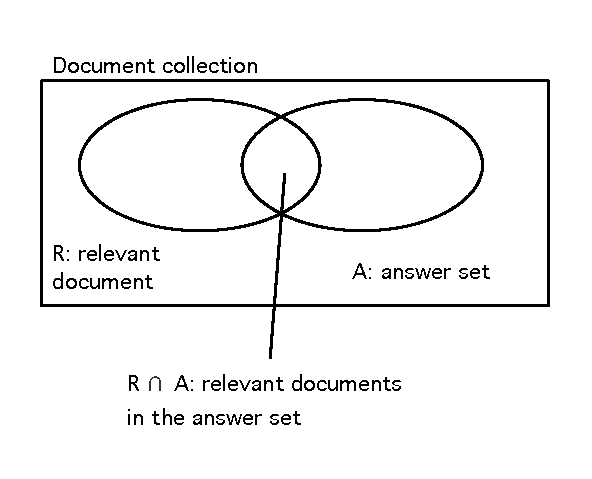
\includegraphics{precision-and-recall.eps}
    \caption{Precision and Recall}
    \label{fig:precisionandrecall}
\end{figure}

จากภาพที่ \ref{fig:precisionandrecall} นั้น อธิบายได้ว่า เมื่อค้นคืนข้อมูลจากคลังเอกสาร (Document collection) แต่ละครั้ง 
จะมีเอกสารที่เกี่ยวข้องกับการค้นคืนในครั้งนั้น ๆ ($R$) อยู่ รวมไปถึงเอกสารที่เป็นคำตอบของระบบ ($A$)
ซึ่งเอกสารคำตอบนั้นอาจเป็นเพียงส่วนหนึ่งหรือเท่ากันกับเอกสารที่เกี่ยวข้อง ($A \subseteq R$) ก็เป็นได้ 
ดังนั้นคำตอบที่ผู้ใช้งานควรจะได้รับจากการค้นคืนคือเอกสารที่เป็นคำตอบและเกี่ยวข้องกับคำค้น ($R \cap A$) ซึ่งการประเมินค่า Recall 
และ Precision นั้น ทำได้ดังนี้

\subsection{Recall \& Precision}

\subsubsection{Recall}

Recall เป็นอัตราส่วนที่ใช้อธิบายถึงความสามารถในการค้นคืนเอกสารที่เกี่ยวข้องจากคลังเอกสาร โดยเทียบระหว่างจำนวนเอกสารที่เป็นคำตอบ
และเกี่ยวข้อง กับจำนวนเอกสารที่ค้นคืนมาได้ ดัง (\ref{eq:recall})

\begin{equation}
    Recall = \frac{|R \cap A|}{|R|}
    \label{eq:recall}
\end{equation}

\subsubsection{Precision}

Precision เป็นอัตราส่วนที่ใช้อธิบายความถูกต้องของการค้นคืนเอกสารว่าสามารถค้นคืนเอกสารที่เกี่ยวข้องขึ้นมาแสดงได้มากน้อยแค่ไหน 
โดยเทียบระหว่างจำนวนเอกสารที่เป็นคำตอบและเกี่ยวข้อง กับจำนวนเอกสารที่เป็นคำตอบ ดัง (\ref{eq:precision})

\begin{align*}
    Precision = \frac{|R \cap A|}{|A|}
    \label{eq:precision}
\end{align*}

\subsubsection{สรุป Recall \& Precision}

Recall และ Precision เป็นการประเมินความแม่นยำของการค้นคืนเอกสารในเบื้องต้น โดยมีข้อจำกัดคือจำเป็นต้องทราบถึงชุดคำตอบ
ของคำค้นอยู่แล้ว ซึ่งมักจะสร้างตารางอธิบายแนวโน้มความถูกต้องบน Recall level ทั้ง 11 ระดับ นั่นคือ 0, 10, 20, 30, 40, 50,
60, 70, 80, 90 และ 100 เพื่อดูแนวโน้มว่าวิธีการค้นคืนที่สนใจอยู่นั้นมีประสิทธิภาพเป็นเช่นไร เช่น ในช่วง Recall level ที่ 0-50\%
วิธีการ ก. นั้นมีมีค่า Precision สูง หากแต่จะลดลงเรื่อยๆ เมื่อมีการแสดงผลลัพธ์มากขึ้น (Recall level สูงกว่า 50\% ขึ้นไป)
หรือใช้เทียบอัตราส่วนโดยดูว่ามีเอกสารที่ถูกต้องมากเท่าใดในเอกสาร 5 หรือ 10 ลำดับแรก (Precision at 5: P@5 
และ Precision at 10: P@10 ตามลำดับ) ซึ่งใช้เพื่อเปรียบเทียบผลลัพธ์ที่ได้จาก Search engine ที่มีปริมาณผลลัพธ์มากๆ 

\subsection{Discounted Cumulated Gain: DCG}
จากการประเมินค่าความถูกต้องของการค้นคืนด้วย Precision และ Recall นั้น จะเห็นได้ว่า ค่าที่ได้นั้นยังเป็นจุดในแต่ละ Recall 
ซึ่งไม่มีความเชื่อมโยงซึ่งกันและกัน Discount cumulated gain (DCG) ขึ้นพัฒนาขึ้นเพื่อรวบรวมคะแนนในแต่ละระดับเพื่อดูถึงประสิทธิผลโดยรวม
ซึ่งต้องพิจารณา 2 ปัจจัยด้วยกันคือ 1) เอกสารที่มีความเกี่ยวข้องมากๆ นั้นมักจะอยู่ในลำดับต้น ๆ 2) เอกสารที่เกี่ยวข้องซึ่งอยู่ในลำดับท้าย ๆ นั้น
ไม่มีความสำคัญเท่าไหร่ โดย DCG นั้นกำหนดระดับความเกี่ยวข้องออกเป็น 4 ระดับด้วยกันคือ 0, 1, 2 และ 3 ซึ่ง 3 แสดงถึงเอกสารนั้น
เกี่ยวข้องมากที่สุด และ 0 คือเอกสารนั้นไม่เกี่ยวข้องเลย โดยมีเงื่อนไขการคำนวณคือ

\begin{equation}
    CG_j[i] = 
    \begin{cases}
        G_j[1]              &; i = 1 > 0 \\
        G_j[i] + CG_j[i-1]  &; otherwise \\
    \end{cases}
    \label{eq:cg}
\end{equation}

เมื่อ $G_i$ คือ ชุดของคะแนนที่ได้ประเมินค่าตามเกณฑ์ของ DCG แล้ว เช่น $G_1$ คือชุดของคะแนนที่ผ่านการประเมินแล้วของเอกสารทั้ง 10 รายการได้แก่ 

\begin{align*}
    G_1 = (1, 0, 1, 0, 3, 2, 1, 0, 0, 2)
\end{align*}

จากนั้นนำ $G_1$ มาคิดหาค่าน้ำหนักรวมโดยพิจารณาจาก (\ref{eq:cg}) จะได้ว่า

\begin{table}[ht!]
    \centering
    \begin{tabular}{rcl} 
        $CG_1$  &=&$(1,$                                      \\
                & &$\,0 + 1,$                                 \\
                & &$\,1 + 0 + 1,$                             \\
                & &$\,0 + 1 + 0 + 1,$                         \\
                & &$\,3 + 0 + 1 + 0 + 1,$                     \\
                & &$\,2 + 3 + 0 + 1 + 0 + 1,$                 \\
                & &$\,1 + 2 + 3 + 0 + 1 + 0 + 1,$             \\
                & &$\,0 + 1 + 2 + 3 + 0 + 1 + 0 + 1,$         \\
                & &$\,0 + 0 + 1 + 2 + 3 + 0 + 1 + 0 + 1,$     \\
                & &$\,2 + 0 + 0 + 1 + 2 + 3 + 0 + 1 + 0 + 1)$ \\
        $CG_1$  &=&$(1, 1, 2, 2, 5, 7, 8, 8, 8, 10)$
    \end{tabular}
\end{table}

จากนั้นนำค่าในชุด $CG_1$ มาทอนด้วยส่วนประกอบเพือลดผลกระทบของค่าคะแนนด้วย (\ref{eq:dcg})

\begin{equation}
    DCG_j[i] = 
    \begin{cases}
        CG_j[1]                                 &; i = 1 > 0 \\
        \frac{CG_j[i]}{\log_2i} + DCG_j[i-1]    &; otherwise \\
    \end{cases}
    \label{eq:dcg}
\end{equation}

จะได้ว่า
\begin{align*}
    DCG_1 = (1.00, 2.00, 2.26, 3.00, 4.15, 7.71, 9.85, 10.67, 10.52, 11.01)
\end{align*}
เมื่อนำค่า $DCG_1$ มาวาดกราฟแล้วจะได้ผลลัพธ์ดังภาพที่ \ref{fig:dcgplot} เพื่อดูแนวโน้มของเอกสาร

\begin{figure}[hbt!]
    \centering
    \begin{tikzpicture}
        \begin{axis}[title={Discounted cumulated gain Graph},
            xlabel={Document},
            ylabel={DCG value},
            xmin=0, xmax=10,
            ymin=0, ymax=12,
            legend pos=north west,
            ]
            \addplot[
                color=blue,
                mark=square,
            ]
            coordinates {
                (1,1.00)(2,2.00)(3,2.26)(4,3.00)(5,4.15)(6,7.71)(7,9.85)(8,10.67)(9,10.52)(10,11.01)
            };
            \legend{$DCG_j$}
        \end{axis}
    \end{tikzpicture}
    \caption{Discount cumulated gain}
    \label{fig:dcgplot}
\end{figure}

ดังนั้น การใช้งาน DCG นั้นก็เพื่อรวบรวมคะแนนความถูกต้องที่ได้ประเมินไปแล้วในหลายๆ ระดับเข้าด้วยกัน 
และช่วยแยกเอกสารที่มีความเกี่ยวข้องมากไว้ด้วย เช่น จาก \figurename\ \ref{fig:dcgplot} เอกสารที่ 5 เป็นเอกสารที่มีความเกี่ยวข้องมากที่สุด 
(พิจารณาจากตำแหน่งก่อนที่กราฟจะมีการเปลี่ยนแปลงความชันมากๆ) 

\end{document} 
